\documentclass[14pt]{beamer}

\usepackage{xcolor}
\usepackage{colortbl}
\usepackage{pgf}
\usepackage{amsmath}
\usepackage{amssymb}
\usepackage{latexsym}
\usepackage{tikz}
\usepackage{pgfplots}
\usepackage{pdfpages}
\usepackage{ulem}

%\includeonlyframes{goal}
\usepackage{rotating}

\usetikzlibrary{positioning, shapes}
\usetikzlibrary{decorations.pathmorphing}

\definecolor{shaded}{RGB}{70,60,255}
\usecolortheme[named=shaded]{structure}

\definecolor{stressed}{RGB}{150,40,40}
\setbeamercolor{alerted_text}{fg=stressed}

\setbeamertemplate{navigation symbols}{}
\setbeamersize{text margin left=3mm} 
\setbeamersize{text margin right=3mm} 

\setbeamertemplate{sidebar right}{default}{}

\makeatletter
\define@key{beamerframe}{nofills}[true]{% top
  \beamer@frametopskip=0pt\relax%
  \beamer@framebottomskip=0pt\relax%
  \beamer@frametopskipautobreak=\beamer@frametopskip\relax%
  \beamer@framebottomskipautobreak=\beamer@framebottomskip\relax%
  \def\beamer@initfirstlineunskip{%
    \def\beamer@firstlineitemizeunskip{%
      \vskip-\partopsep\vskip-\topsep\vskip-\parskip%
      \global\let\beamer@firstlineitemizeunskip=\relax}%
    \everypar{\global\let\beamer@firstlineitemizeunskip=\relax}}
}
\makeatother

\newcommand{\defnword}[1]{\textbf{#1}}

\usepackage{amsthm}
\newtheorem*{conjecture}{Conjecture}

\newtheorem{observation}[theorem]{Observation}
%\newtheorem{definition}[theorem]{Definition}
\newtheorem{remark}[theorem]{Remark}
\newtheorem{claim}[theorem]{Claim}
\newtheorem{proposition}[theorem]{Proposition}
\newtheorem{question}[theorem]{Question}

\newcommand{\Z}{\mathbb{Z}}
\newcommand{\Q}{\mathbb{Q}}
\newcommand{\R}{\mathbb{R}}
\newcommand{\OO}{\mathbb{O}}
\newcommand{\HH}{\mathbb{H}}
\newcommand{\RP}{\mathbb{R}P}
\newcommand{\CP}{\mathbb{C}P}
\newcommand{\HP}{\mathbb{H}P}
\newcommand{\OP}{\mathbb{O}P}
\DeclareMathOperator{\Spin}{Spin}
\DeclareMathOperator{\Homeo}{Homeo}
\DeclareMathOperator{\SO}{SO}
\DeclareMathOperator{\fiber}{fiber}
\DeclareMathOperator{\proj}{proj}

\newcommand{\LL}{\mathbb{L}}
\newcommand{\setbackgroundblack}{%
\usebackgroundtemplate{
\begin{pgfpicture}{0in}{0in}{\paperwidth}{\paperheight}
\color{black}
\pgfrect[fill]{\pgfxy(0,0)}{\pgfpoint{\paperwidth}{\paperheight}}
\end{pgfpicture}
}
}

\newcommand{\setbackgroundgreen}{%
\usebackgroundtemplate{
\begin{pgfpicture}{0in}{0in}{\paperwidth}{\paperheight}
\color{red!50!black}
\pgfrect[fill]{\pgfxy(0,0)}{\pgfpoint{\paperwidth}{\paperheight}}
\end{pgfpicture}
}
}

\newcommand{\sectionslide}[1]{%
\setbackgroundblack
\begin{frame}[nofills]
\Huge
\vfill
\scaletowidth{\textwidth}{\textcolor{white}{\textbf{#1}}}
\vfill
\end{frame}
\clearbackgroundpicture
}

\newcommand{\encouragement}[1]{%
\setbackgroundgreen
\begin{frame}[nofills]
\Huge
\vfill
\scaletowidth{\textwidth}{\textcolor{white}{#1}}
\vfill
\end{frame}
\clearbackgroundpicture
}

\definecolor{FootColor}{rgb}{0.322,0.322,0.322}%
\definecolor{FootBackgroundColor}{rgb}{1,1,1}%

\setbeamercolor{bottomcolor}{fg=black,bg=gray!15!white}

%\setbeamertemplate{footline}{%
%\usebeamerfont{structure}
%\footnotesize
%\begin{tikzpicture}[overlay,remember picture]%
%  \node[opacity=0.8,text opacity=1,anchor=base west,yshift=2pt,xshift=-0.5mm,color=FootColor,fill=FootBackgroundColor] (website) at (current page.south west) {mooculus.osu.edu};
%  \node[opacity=0.8,text opacity=1,anchor=base east,yshift=2pt,xshift=0.5mm,color=FootColor,fill=FootBackgroundColor] (twitter) at (current page.south east) {\#mooculus};
%\end{tikzpicture}
%}

%%%%%%%%%%%%%%%%%%%%%%%%%%%%%%%%%%%%%%%%%%%%%%%%%%%%%%%%%%%%%%%%
% stack two things so that they have the same size
\newlength{\firstline}
\newlength{\secondline}
\newcommand{\stacksame}[2]{%
\setlength{\firstline}{\widthof{#1}}%
\setlength{\secondline}{\widthof{#2}}%
\pgfmathsetmacro{\myratio}{\firstline/\secondline}%
\shortstack{#1\\\scalebox{\myratio}{#2}}}

\newlength{\myscalewidth}
\newcommand{\scaletowidth}[2]{%
\setlength{\myscalewidth}{\widthof{#2}}%
\pgfmathsetmacro{\myscaleratio}{#1/\myscalewidth}%
\scalebox{\myscaleratio}{#2}}


%%%%%%%%%%%%%%%%%%%%%%%%%%%%%%%%%%%%%%%%%%%%%%%%%%%%%%%%%%%%%%%%
% I like words in front of faded images

\newcommand{\setbackgroundpicturewhite}[1]{%
\definecolor{FootColor}{rgb}{0.322,0.322,0.322}%
\definecolor{FootBackgroundColor}{rgb}{1,1,1}%
\setbeamercolor{bottomcolor}{fg=black,bg=gray!15!white}%
\usebackgroundtemplate{%
\begin{tikzpicture}[overlay,remember picture]%
\draw[fill=white] (current page.north west) rectangle (current page.south east);%
\node[fill=white,minimum width=\paperwidth,minimum height=\paperheight,yshift=1.5mm] [anchor=north west] (mynode) {\hspace{-1.5mm}\includegraphics[width=\paperwidth]{#1}};%
\end{tikzpicture}%
}}


\newcommand{\settallbackgroundpicturewhite}[1]{%
\definecolor{FootColor}{rgb}{0.322,0.322,0.322}%
\definecolor{FootBackgroundColor}{rgb}{1,1,1}%
\setbeamercolor{bottomcolor}{fg=black,bg=gray!15!white}%
\usebackgroundtemplate{%
\begin{tikzpicture}[overlay,remember picture]%
\draw[fill=white] (current page.north west) rectangle (current page.south east);%
\node[minimum width=\paperwidth,minimum height=\paperheight,yshift=1.5mm] [anchor=north west] (mynode) {\hspace{-1.5mm}\includegraphics[height=\paperheight]{#1}};%
\end{tikzpicture}%
}}


\newcommand{\settallbackgroundpictureblack}[1]{%
\definecolor{FootColor}{rgb}{0.678,0.678,0.678}%
\definecolor{FootBackgroundColor}{rgb}{0,0,0}%
\setbeamercolor{bottomcolor}{fg=black,bg=gray!15!white}%
\usebackgroundtemplate{%
\begin{tikzpicture}[overlay,remember picture]%
\draw[fill=black] (current page.north west) rectangle (current page.south east);%
\node[minimum width=\paperwidth,minimum height=\paperheight,yshift=1.5mm] [anchor=north west] (mynode) {\hspace{-1.5mm}\includegraphics[height=\paperheight]{#1}};%
\end{tikzpicture}%
}}


\newcommand{\setbackgroundpictureblack}[1]{%
\definecolor{FootColor}{rgb}{0.678,0.678,0.678}%
\definecolor{FootBackgroundColor}{rgb}{0,0,0}%
\setbeamercolor{bottomcolor}{fg=white,bg=gray!15!black}%
\usebackgroundtemplate{%
\begin{tikzpicture}[overlay,remember picture]%
\draw[fill=black] (current page.north west) rectangle (current page.south east);%
\node[minimum width=\paperwidth,minimum height=\paperheight,yshift=1.5mm] [anchor=north west] (mynode) {\hspace{-1.5mm}\includegraphics[width=\paperwidth]{#1}};%
\end{tikzpicture}%
}}


\newcommand{\setdarkbackgroundpictureblack}[1]{%
\definecolor{FootColor}{rgb}{0.678,0.678,0.678}%
\definecolor{FootBackgroundColor}{rgb}{0,0,0}%
\setbeamercolor{bottomcolor}{fg=white,bg=gray!15!black}
\usebackgroundtemplate{%
\begin{tikzpicture}[overlay,remember picture]%
\draw[fill=black] (current page.north west) rectangle (current page.south east);%
\node[minimum width=\paperwidth,minimum height=\paperheight,yshift=1.5mm] [anchor=north west] (mynode) {\hspace{-1.5mm}\includegraphics[width=\paperwidth]{#1}};%
\draw[fill=black,opacity=0.75] (current page.north west) rectangle (current page.south east);%
\end{tikzpicture}%
}}%


\newcommand{\setdarkbackgroundpicturewhite}[1]{%
\definecolor{FootColor}{rgb}{0.322,0.322,0.322}%
\definecolor{FootBackgroundColor}{rgb}{1,1,1}%
\setbeamercolor{bottomcolor}{fg=black,bg=gray!15!white}
\usebackgroundtemplate{%
\begin{tikzpicture}[overlay,remember picture]%
\draw[fill=white] (current page.north west) rectangle (current page.south east);%
\node[minimum width=\paperwidth,minimum height=\paperheight,yshift=1.5mm] [anchor=north west] (mynode) {\hspace{-1.5mm}\includegraphics[width=\paperwidth]{#1}};%
\draw[fill=white,opacity=0.75] (current page.north west) rectangle (current page.south east);%
\end{tikzpicture}%
}}%

\newcommand{\settalldarkbackgroundpicturewhite}[1]{%
\definecolor{FootColor}{rgb}{0.322,0.322,0.322}%
\definecolor{FootBackgroundColor}{rgb}{1,1,1}%
\setbeamercolor{bottomcolor}{fg=black,bg=gray!15!white}
\usebackgroundtemplate{%
\begin{tikzpicture}[overlay,remember picture]%
\draw[fill=white] (current page.north west) rectangle (current page.south east);%
\node[minimum width=\paperwidth,minimum height=\paperheight,yshift=1.5mm] [anchor=north west] (mynode) {\hspace{-1.5mm}\includegraphics[height=\paperheight]{#1}};%
\draw[fill=white,opacity=0.75] (current page.north west) rectangle (current page.south east);%
\end{tikzpicture}%
}}%


\newcommand{\settalldarkbackgroundpictureblack}[1]{%
\definecolor{FootColor}{rgb}{0.678,0.678,0.678}%
\definecolor{FootBackgroundColor}{rgb}{0,0,0}%
\setbeamercolor{bottomcolor}{fg=black,bg=gray!15!white}
\usebackgroundtemplate{%
\begin{tikzpicture}[overlay,remember picture]%
\draw[fill=black] (current page.north west) rectangle (current page.south east);%
\node[minimum width=\paperwidth,minimum height=\paperheight,yshift=1.5mm] [anchor=north west] (mynode) {\hspace{-1.5mm}\includegraphics[height=\paperheight]{#1}};%
\draw[fill=black,opacity=0.75] (current page.north west) rectangle (current page.south east);%
\end{tikzpicture}%
}}%

\newcommand{\clearbackgroundpicture}{\usebackgroundtemplate{}%
\definecolor{FootColor}{rgb}{0.322,0.322,0.322}%
\definecolor{FootBackgroundColor}{rgb}{1,1,1}%
\setbeamercolor{bottomcolor}{fg=black,bg=gray!15!white}
}

\definecolor{osugray}{HTML}{5e6061}
\definecolor{ccgray}{HTML}{a7b1a6}

\newcommand{\whitebackground}{\setbeamercolor{background canvas}{bg=white,fg=black}\usebeamercolor[fg]{background canvas}}
\newcommand{\blackbackground}{\setbeamercolor{background canvas}{bg=black,fg=white}\usebeamercolor[fg]{background canvas}}

\begin{document}
\whitebackground

%%%%%%%%%%%%%%%%%%%%%%%%%%%%%%%%%%%%%%%%%%%%%%%%%%%%%%%%%%%%%%%%
\clearbackgroundpicture
\begin{frame}[nofills]
  \vspace{5ex}

  \large
  \scaletowidth{\textwidth}{\textbf{Ximera}}

  \vfill
  
  \color{osugray}

  \begin{columns}
    \begin{column}{0.3\textwidth}
      \vfill
      \scriptsize
      \vspace{-6ex}
      \scaletowidth{\textwidth}{PCCIW} \\[1ex]
      \scaletowidth{\textwidth}{November 13, 2015}

    \end{column}
    \hfill
    \begin{column}{0.65\textwidth}
      \vfill
      \vspace{2.5ex}
      \normalsize
      \textsf{\textbf{Jim Fowler and Steve Gubkin}} \\
      \textsf{The Ohio State University} \\
      \textsf{Department of Mathematics} \\
      \vspace{0.6in}
\end{column}
\end{columns}
  
\end{frame}

%%%%%%%%%%%%%%%%%%%%%%%%%%%%%%%%%%%%%%%%%%%%%%%%%%%%%%%%%%%%%%%%
\clearbackgroundpicture
\begin{frame}
  \frametitle{Joint Work}
  \large 

  Joint work with \\
  \quad Herb Clemens and Bart Snapp \\
  \quad and now many others in \\
  \quad\quad the Ohio State math department.

  \vfill

  Funded by \\
  \quad NSF DUE--1245433 and \\
  \quad NSF DUE--1505246.

\end{frame}

\encouragement{MOOCs}

%%%%%%%%%%%%%%%%%%%%%%%%%%%%%%%%%%%%%%%%%%%%%%%%%%%%%%%%%%%%%%%%
% The MOOCs
\begin{frame}
  \begin{tikzpicture}[overlay,remember picture]
    \uncover<1>{
      \node[anchor=north west,rotate=0,xshift=0pt,yshift=0pt] (label) at (current page.north west) {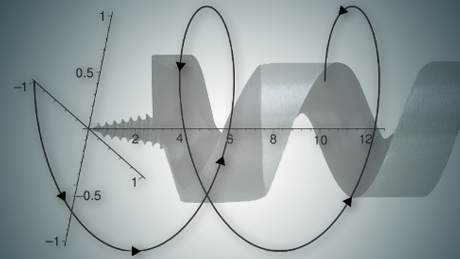
\includegraphics[width=0.4\textwidth]{logos/calculus-one.png}};
      \node[anchor=west,rotate=0,xshift=0pt,yshift=0pt] (label) at (current page.west) {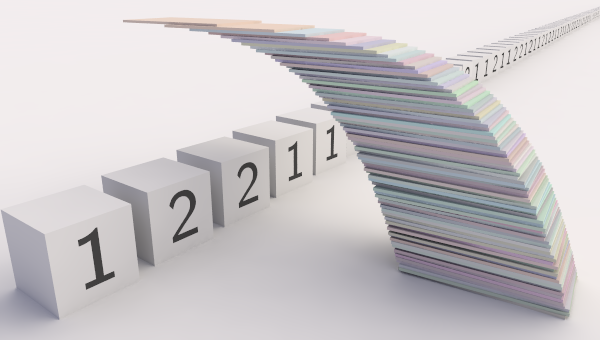
\includegraphics[width=0.4\textwidth]{logos/calculus-two.png}};
      \node[anchor=south west,rotate=0,xshift=0pt,yshift=0pt] (label) at (current page.south west) {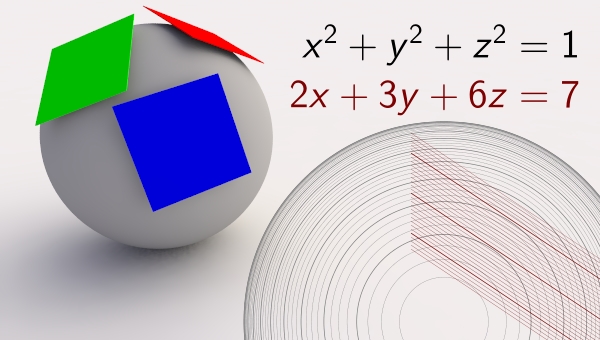
\includegraphics[width=0.4\textwidth]{logos/m2o2c2.png}};

      \node[anchor=west,rotate=0,xshift=0.5\textwidth,yshift=-0.11304\textwidth] (label) at (current page.north west) {Calculus One};
      \node[anchor=west,rotate=0,xshift=0.5\textwidth,yshift=0pt] (label) at (current page.west) {\parbox{0.5\textwidth}{Calculus Two:\\ Sequences and Series}};
      \node[anchor=west,rotate=0,xshift=0.5\textwidth,yshift=0.11304\textwidth] (label) at (current page.south west) {\parbox{0.5\textwidth}{M2O2C2:\\ Massively Multivariable Open Online Calculus Course}};
    }
  \end{tikzpicture}
\end{frame}

\encouragement{Face-to-face?}

%%%%%%%%%%%%%%%%%%%%%%%%%%%%%%%%%%%%%%%%%%%%%%%%%%%%%%%%%%%%%%%%
\clearbackgroundpicture
\begin{frame}
  \Large

  \frametitle{Calculus interventions}

  Ohio State's math department \\
  \quad is studying various interventions \\
  \quad to improve outcomes in Calculus 1.

  \vfill

  Bart Snapp's section uses the \\
  \quad open-source Ximera-based text (IIIS), \\
  while other sections \\
  \quad use the commercial text.

  \vfill

  %pre- and post-test on concepts
\end{frame}

\clearbackgroundpicture
\begin{frame}[nofills]
  \vspace{1ex}
  \Huge
  
\includegraphics[width=\textwidth]{images/cow.pdf}
  \vfill
  \pause
  \Large
  \scaletowidth{\textwidth}{cow-culus}
  \vfill
  \scaletowidth{\textwidth}{\url{https://github.com/mooculus/mooculus}}
\end{frame}

%%%%%%%%%%%%%%%%%%%%%%%%%%%%%%%%%%%%%%%%%%%%%%%%%%%%%%%%%%%%%%%%
\begin{frame}
  \frametitle{Evaluation}
  \large

  \begin{itemize}
  \item Demographic and placement data
  \item Surveys from Bressoud's study
  \item Common midterms and finals
  \item Website engagement analytics
  \end{itemize}
\end{frame}

%%%%%%%%%%%%%%%%%%%%%%%%%%%%%%%%%%%%%%%%%%%%%%%%%%%%%%%%%%%%%%%%
\begin{frame}
  \frametitle{Pre- and post-test}

  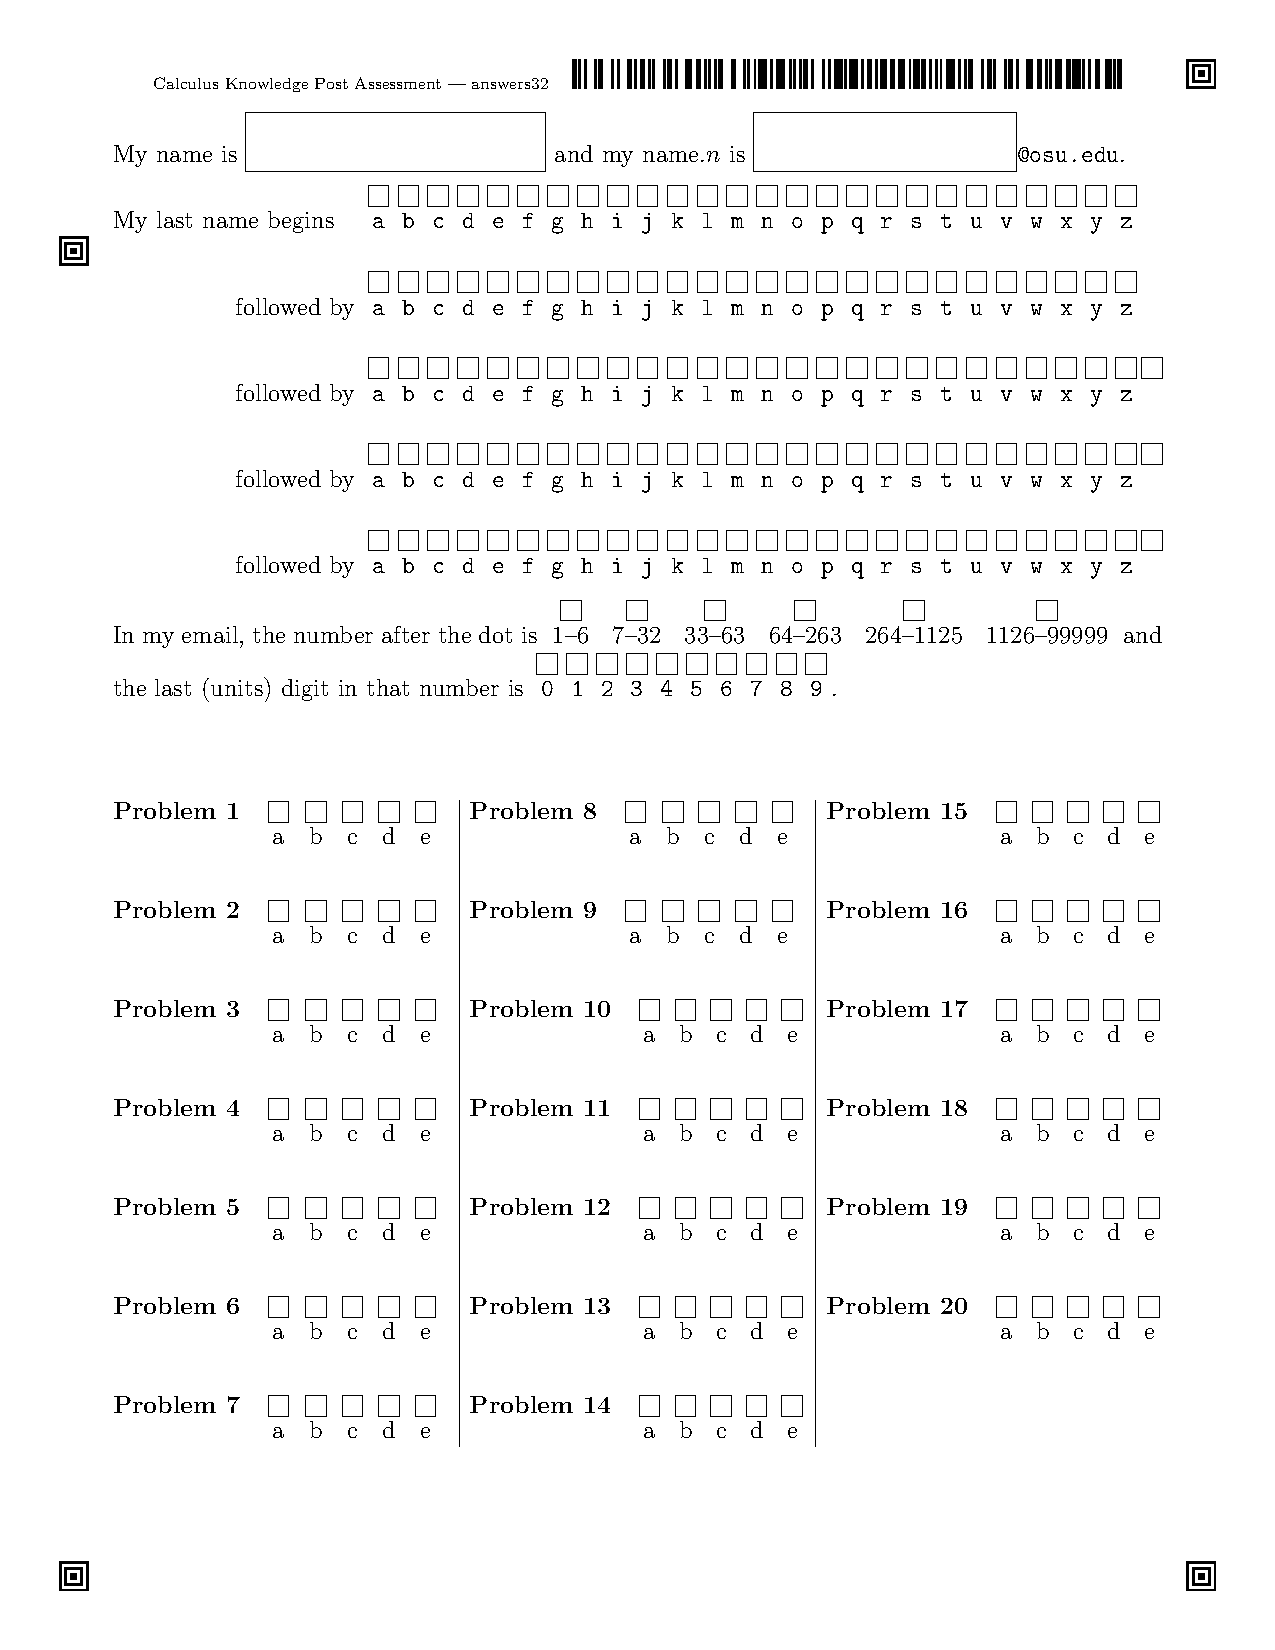
\includegraphics[width=\textwidth]{images/pretest.pdf}
\end{frame}

\begin{frame}
  \large
  \frametitle{Dogfooding Ximera}

  % Ximera is the open platform.
  % Content from GitHub is automatically served on the web.

  Ohio State's math department \\
  \quad started with an open-source calculus text \\
  \quad\quad written in the 1990s \\
  \quad and has edited it \\
  \quad\quad collaboratively via GitHub.

\end{frame}

%%%%%%%%%%%%%%%%%%%%%%%%%%%%%%%%%%%%%%%%%%%%%%%%%%%%%%%%%%%%%%%%
\begin{frame}
  \frametitle{Theory of Change}

  \begin{itemize}
  \item Learning outcomes (``backwards design'')
  \item Education seminar within math department
  \item Many local authors for broad buy-in
  \item Card system (Trello) to organize work
  \item Calculus coordinators
  \item Calculus Czar (John Johnson)
  \end{itemize}

\end{frame}

%%%%%%%%%%%%%%%%%%%%%%%%%%%%%%%%%%%%%%%%%%%%%%%%%%%%%%%%%%%%%%%%
\encouragement{Requirements}

\begin{frame}
  \frametitle{User stories}
  
  \begin{itemize}
    \item Everyone commits to ``open.''
    \item Content creators act like software engineers.
    \item Students' experience should be engaging.
    \item Instructors get data.
  \end{itemize}
\end{frame}

%%%%%%%%%%%%%%%%%%%%%%%%%%%%%%%%%%%%%%%%%%%%%%%%%%%%%%%%%%%%%%%%
\begin{frame}
  \frametitle{Commitment to Open}
  \Large 

  Backend technology is open \\
  \quad with GPLv3 license.

  Mathematical content is open, \\
  \quad with CC-BY-SA license.

\end{frame}

%%%%%%%%%%%%%%%%%%%%%%%%%%%%%%%%%%%%%%%%%%%%%%%%%%%%%%%%%%%%%%%%
\begin{frame}
  \frametitle{Content creators and editors}

  \begin{itemize}
  \item Plain text %$\Doublerightarrow$
  \item Version control
  \item Branches: development versus master
  \item A/B testing
  \item Text editor
  \item Leverage existing technology (e.g., \LaTeX).
  \end{itemize}

\end{frame}

%%%%%%%%%%%%%%%%%%%%%%%%%%%%%%%%%%%%%%%%%%%%%%%%%%%%%%%%%%%%%%%%
\begin{frame}
  \frametitle{Student experience}

  Content interweaves ``homework'' and ``textbook'' \\
  \quad into ``activities'' (tasks, worksheets).

  \vfill\pause

  Students can look under the hood.

  \vfill\pause
  
  Interactive JavaScript means \\
  \quad the browser is doing the heavy-lifting, \\
  \quad and the experience is low-latency.
  
\end{frame}

%%%%%%%%%%%%%%%%%%%%%%%%%%%%%%%%%%%%%%%%%%%%%%%%%%%%%%%%%%%%%%%%
% Mobile
\clearbackgroundpicture
\usebackgroundtemplate{%
\begin{tikzpicture}[overlay,remember picture]%
\draw[fill=black] (current page.north west) rectangle (current page.south east);%
\node[minimum width=\paperwidth,minimum height=\paperheight,yshift=1.5mm] [anchor=north west] (mynode) {};%
\draw[fill=black,opacity=0.75] (current page.north west) rectangle (current page.south east);%
\end{tikzpicture}%
}
\begin{frame}
  \blackbackground
  \begin{columns}
    \begin{column}{0.5\textwidth}
      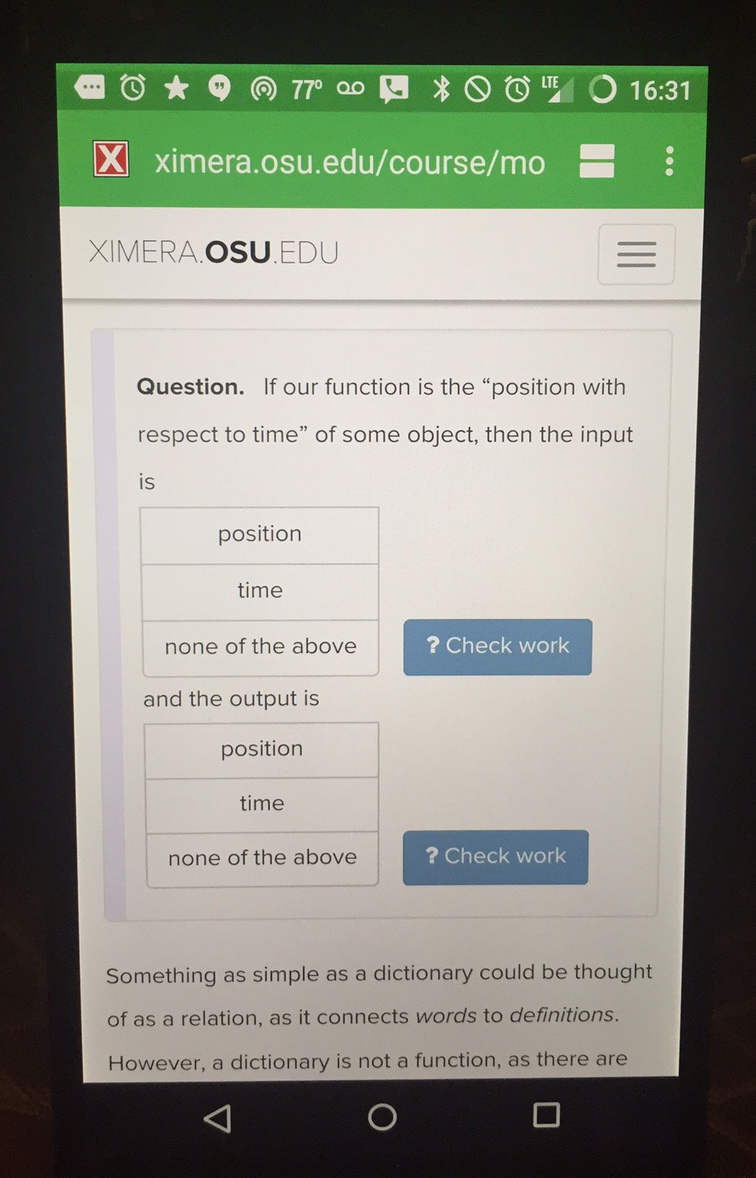
\includegraphics[width=\textwidth]{ximera/mobile.jpg}
    \end{column}
    \begin{column}{0.5\textwidth}
      \vfill
      \color{white}
      \scaletowidth{\textwidth}{Mobile}
      \vfill
    \end{column}
  \end{columns}
\end{frame}

\clearbackgroundpicture
\begin{frame}
  \frametitle{Instructors need data}

  Rely on a ``Learning Record Store'' like \\
  \quad the Experience API (Tin Can) or \\
  \quad Caliper, \\
  and provide a dashboard with export to R.

  \vfill\pause

  Don't rely on randomization \\
  \quad because randomization stands in tension \\
  \quad with data analysis.

\end{frame}

\encouragement{Requirements}

\begin{frame}
  \frametitle{Requirements}
  \Large

  \begin{itemize}
  \item Open
  \item Software Engineering
  \item Engaging
  \item Data
  \end{itemize}
\end{frame}

\begin{frame}[nofills]
  \frametitle{What is Ximera?}

  \vspace{-0.35in}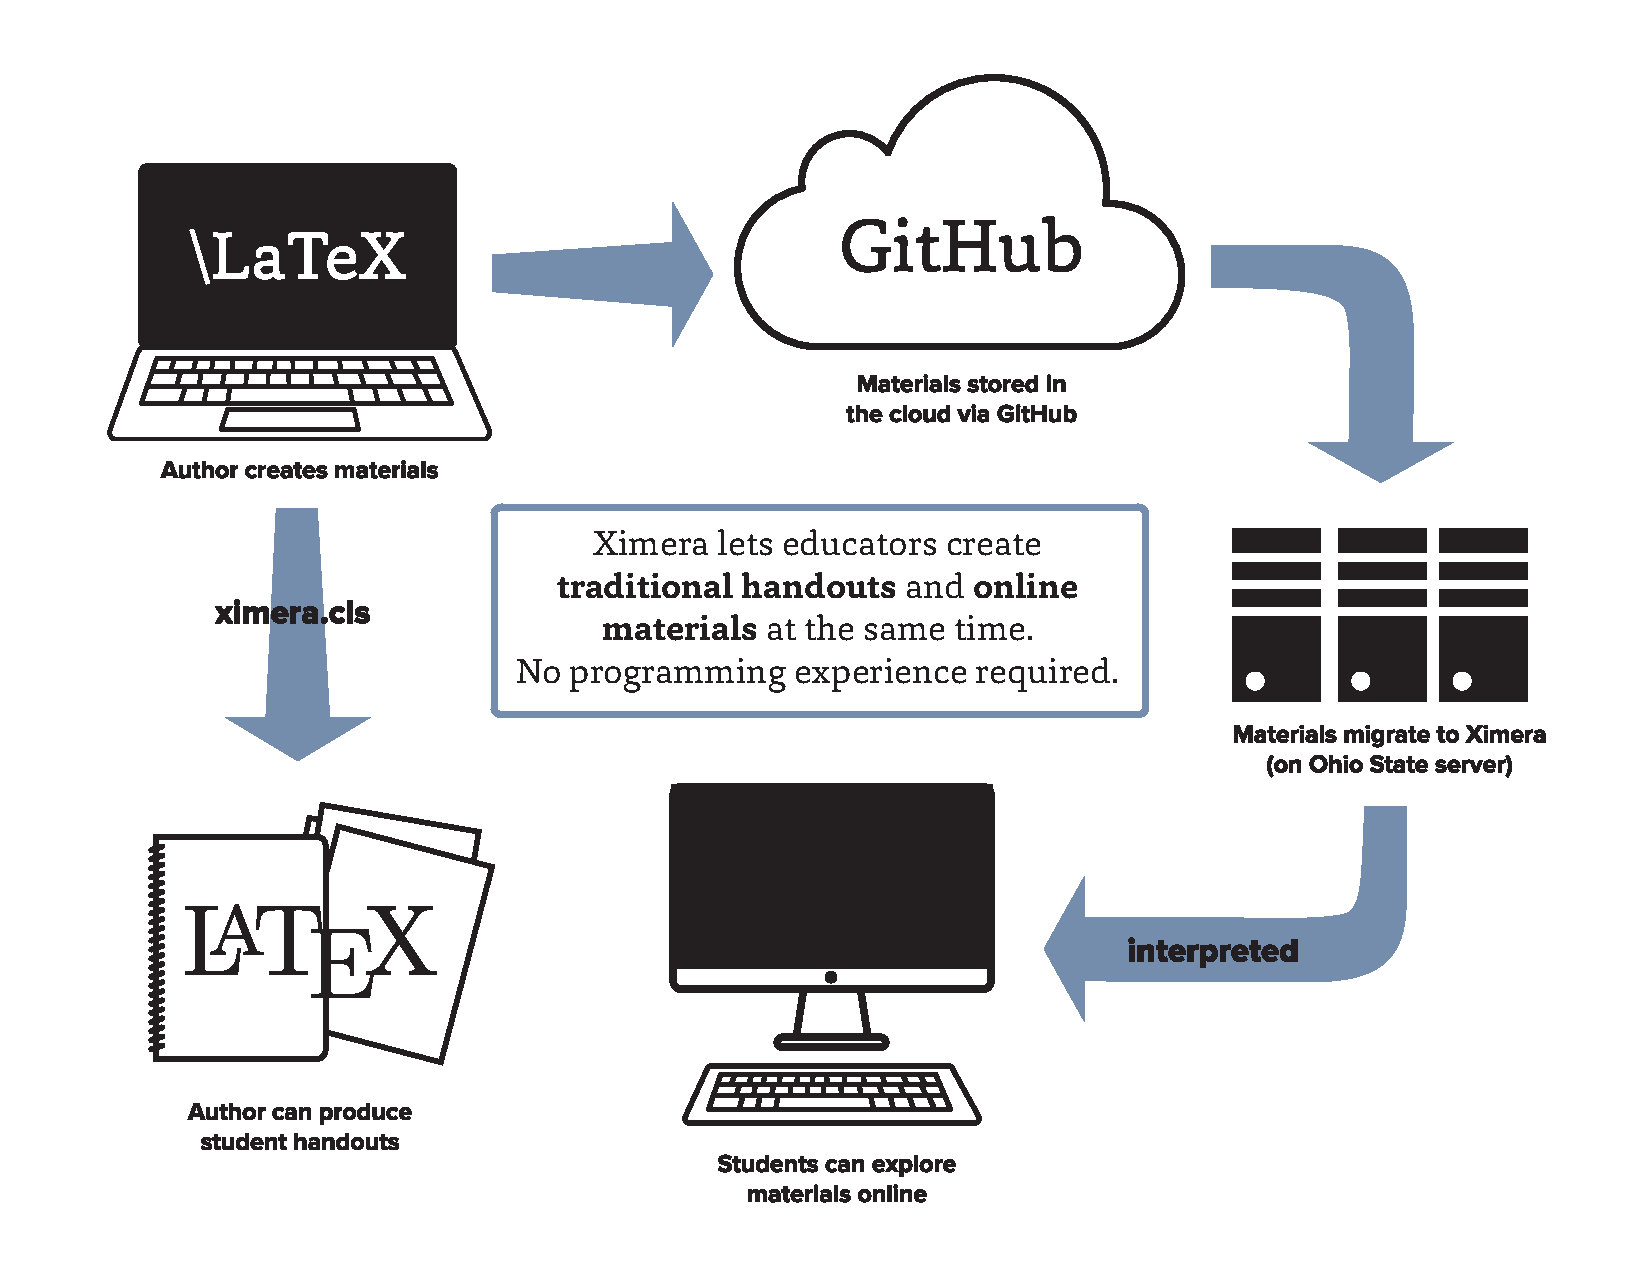
\includegraphics[width=\textwidth]{ximera/infographic.pdf}
\end{frame}

\encouragement{Let's see it!}

%%%%%%%%%%%%%%%%%%%%%%%%%%%%%%%%%%%%%%%%%%%%%%%%%%%%%%%%%%%%%%%%
\setbackgroundpictureblack{ximera/ximera-calculus.png}
\begin{frame}
\end{frame}

\setdarkbackgroundpictureblack{ximera/ximera-calculus.png}
\begin{frame}[nofills]
\vfill\color{white}
\begin{center}
\Huge\textsf{\textbf{\scaletowidth{0.75\textwidth}{\stacksame{Calculus}{content}}}}
\end{center}
\vfill
\end{frame}

%%%%%%%%%%%%%%%%%%%%%%%%%%%%%%%%%%%%%%%%%%%%%%%%%%%%%%%%%%%%%%%%
\setbackgroundpictureblack{ximera/ximera-multiple-choice.png}
\begin{frame}
\end{frame}

\setdarkbackgroundpictureblack{ximera/ximera-multiple-choice.png}
\begin{frame}[nofills]
\vfill\color{white}
\begin{center}
\Huge\textsf{\textbf{\scaletowidth{0.75\textwidth}{\stacksame{multiple}{choice}}}}
\end{center}
\vfill
\end{frame}



%%%%%%%%%%%%%%%%%%%%%%%%%%%%%%%%%%%%%%%%%%%%%%%%%%%%%%%%%%%%%%%%
\setbackgroundpictureblack{ximera/ximera-math-answer.png}
\begin{frame}
\end{frame}

\setdarkbackgroundpictureblack{ximera/ximera-math-answer.png}
\begin{frame}[nofills]
\vfill\color{white}
\begin{center}
\Huge\textsf{\textbf{\scaletowidth{0.75\textwidth}{\stacksame{mathematical}{expressions}}}}
\end{center}
\vfill
\end{frame}


 %%%%%%%%%%%%%%%%%%%%%%%%%%%%%%%%%%%%%%%%%%%%%%%%%%%%%%%%%%%%%%%%
 \clearbackgroundpicture
 \begin{frame}[label=thanks,nofills]
   \vfill
   \begin{center}
   \Huge
    \scalebox{1.5}{\textbf{Thank You}}
   \end{center}
   \vfill
   \begin{center}
     \url{https://github.com/kisonecat/pcciw}
   \end{center}
   \vfill
   
\includegraphics[width=1in]{images/cc-logo.pdf}\hfill\footnotesize\scalebox{0.75}{\textcolor{ccgray}{Licensed for reuse under a Creative Commons BY-NC-SA License}}
   \null
   %\vspace{12pt}
   \null
 \end{frame}

\begin{frame}
  \Large

  The choice is not \\
  \quad zero versus non-zero price.

  The choice is between \\
  \quad open versus closed. 

  \large
  \vfill\pause
  \begin{tabular}{l@{ }l@{ }l}
    What does & a closed & textbook say about learning? \pause\\
    &an open& textbook 
  \end{tabular}
  
\end{frame}



\end{document}
